\documentclass[sigconf,review,anonymous]{acmart}

\usepackage{booktabs}
\usepackage{siunitx}
\usepackage{xurl}

\setcopyright{none}
\acmConference[WWW '27]{Proceedings of the ACM Web Conference 2027}{May 10--14, 2027}{Dublin, Ireland}
\acmYear{2027}
\acmDOI{}
\acmISBN{}
\settopmatter{printacmref=false}
\renewcommand\footnotetextcopyrightpermission[1]{}

\begin{document}

\title{Budget, Readout or Reasoning? Where Small Reasoning Models Lose Value in Auction Bidding}

\author{Anonymous Author(s)}
\affiliation{\institution{Anonymous Institution}\country{}}

\begin{abstract}
Ad platforms and marketplaces show bidders a bid landscape, the estimated chance of winning at each candidate bid, and increasingly let agents built on reasoning language models choose the bid. We give six open reasoning models such landscapes, with win curves from eBay prices and from a simulated ad market (AuctionNet), and score their bids against an exact calculator. Two failures belong to the models. They pass over the best option that their own trace has already computed and ranked first, and their wrong answers lean toward the highest bid on the menu, which costs bidders 7--17\% of the calculator's surplus under pay-your-bid pricing. Arithmetic errors are rare. Two further losses come from operator choices. A token cap cuts traces short: allowed to stop on their own within 4{,}096 tokens, five models recover 91--100\% of the calculator's lead over no reasoning. Asking for the answer while the reasoning block is still open misreads it: closing the block first lifts the weakest model from 42\% to 84\%. An audit that flags bids disagreeing with the trace's own numbers for override recovers 84--100\% of the loss under nested cross-validation.
\end{abstract}

\ccsdesc[500]{Applied computing~Online auctions}
\ccsdesc[300]{Information systems~Computational advertising}
\ccsdesc[300]{Computing methodologies~Natural language processing}

\keywords{web economics, bid landscape, test-time compute, LLM agents, online auctions, inference cost}

\maketitle

\section{Introduction}

Much of the web's commerce is priced by automated auction, and platforms increasingly hand the bidder the forecast. Ad platforms and marketplaces expose a bid landscape or win-rate simulator, the estimated chance of winning at each candidate bid, and leave the choice of bid to the advertiser, seller or buyer, or to an agent acting for them. The Web challenge is delegated bidding: as platforms let reasoning-model agents act on bid landscapes, operators must decide how much reasoning to pay for and how to check an agent's bid. (Track: Web Economics and Digital Society.) These choices are made per keyword, campaign or high-value listing, not per impression, so an agent can spend seconds on each. LLM agents are being built to bid, price and negotiate in such markets \cite{chen2024aucarena,zhu2024synthetic,ahmed2026bazaar}, increasingly on reasoning models that spend tokens before acting. This paper asks where the value of reasoning tokens is lost in the bid-landscape decision, and what the wrong bids look like.

The task is deliberately easy, and that is the point: because the agent receives the estimates, an exact calculator solves it, so every lost dollar can be traced to the agent's reasoning, its answer, or our forcing and read-out protocol. Why not let the calculator bid? Deployed agents do not face a calculator-sized problem. The landscape is one input among others the calculator cannot weigh, such as budget pacing, brand goals or the advertiser's notes, and the operator, often a company running a vendor's agent or a platform hosting third-party agents, can read the agent's reasoning but cannot replace it. An agent that loses value on the one step a calculator can check is unlikely to do better once that step sits inside a richer decision, so we treat its loss as a lower bound, and ask which bids the operator should flag for review or override. The target setting is a pay-your-bid auction in which an agent sets the bid for a keyword, a campaign or a high-value listing from a landscape; first-price rules have spread in ad auctions \cite{despotakis2021firstprice}. eBay runs proxy bidding instead, and we do not model its rule: its closing prices only supply realistic empirical shapes for the win curves.

Code, saved decisions and scripts are in an anonymous repository.\footnote{\url{https://anonymous.4open.science/r/reasoning-compute-economic-utility-EED7/}}



\section{Related work}

Test-time scaling trades tokens for accuracy \cite{wei2022chain,snell2024scaling}; our forcing resembles budget forcing \cite{muennighoff2025s1}. Reasoning models can overthink \cite{chen2024overthinking} or abandon promising lines \cite{wang2025underthinking}. Answers depend on option order \cite{zheng2024mcq,pezeshkpour2024order} and need not follow the stated reasoning \cite{turpin2023unfaithful,lanham2023faithfulness,chen2025reasoningsay}; we measure both in dollars. Tool-using models offload arithmetic \cite{schick2023toolformer}. Bid landscapes are forecast from auction logs \cite{cui2011bidlandscape} and feed auto-bidding \cite{aggarwal2024autobidding}, where LLMs now act as bidding agents \cite{cai2025rtbagent} or reasoning modules \cite{li2026lbm}; \citet{duetting2024mechanism} design auctions among LLM agents. LLM agents have been studied as bidders and economic actors \cite{chen2024aucarena,zhu2024synthetic,ahmed2026bazaar,raman2024steer,fish2025econevals}; unlike EconEvals \cite{fish2025econevals} and STEER \cite{raman2024steer}, which score whether decisions are rational, we locate where a trace loses value it has already computed.

\section{Task, models and measurement}

\paragraph{Scenarios}
We use 628 eBay auctions of Palm Pilot PDAs, Xbox consoles and Cartier watches collected by Jank and Shmueli \cite{jank2010modeling}, in the Kaggle copy \cite{onlineauctionsdataset}, split 70/30 within product. Per product, 18 private values $v$ are spaced evenly from the 35th percentile of construction-sample closing prices to 1.25 times the 95th. For each value and menu size $K\in\{5,7\}$, two candidate sets of \$5-step bids are drawn below $v$ within the 2nd--98th price percentiles, as a random contiguous window or a random sample, never conditioned on the optimum: 216 scenarios. Each bid shows $\hat p(b)$, the share of construction prices at or below $b$; the chosen bid is scored with the same estimator on the 189 held-out auctions. These are realistic empirical win curves rather than first-price win rates; models and calculator see the same landscape.

\emph{AuctionNet.} To test a second market we rebuilt the task on AuctionNet \cite{su2024auctionnet}, a simulated ad market in which 48 auto-bidding agents compete in a three-slot generalized second-price auction over generated ad traffic. The competing price of an opportunity is the third-highest rival bid; products are terciles of conversion probability, bids are per 1{,}000 impressions, win curves come from periods 7--9 and scoring from period 10, and 216 scenarios are built as above (step 2). As on eBay, a bid is scored pay-your-bid, $p(b)(v-b)$, with $p(b)$ the share of held-out opportunities whose competing price is at most $b$; we do not model GSP payments or slot exposure. These runs used vLLM on an L40S, which on eBay moves Phi-mini's and Granite-8B's $q$ by at most 0.027.

\paragraph{Measures}
\emph{Utility ratio} $q=U(\hat b)/\max_b U(b)$ with expected profit $U(b)=p(b)(v-b)$ under held-out probabilities $p$. The calculator returns $\arg\max_b \hat p(b)(v-b)$ and scores $q=0.981$; random choice scores 0.711. Our primary measure, \emph{gap recovered} at budget $c$, is $(q(c)-q(0))/(q_{\text{calc}}-q(0))$, averaged per decision; $q(0)$ is the same model, prompt and readout with no reasoning tokens, so the measure isolates what the tokens buy. Pooling dollars instead weights the costliest product most and is reported as secondary. Intervals resample the 18 value families within each product (2{,}000 draws). For a second scoring curve (\emph{FP eq.}) rivals bid the symmetric first-price equilibrium for a lognormal value distribution fitted to each product's closing prices, read as second-highest values.

\paragraph{Models and protocol}
The checkpoints are Phi-4-mini-reasoning (Phi-mini), Qwen3-4B, -8B and -14B, DeepSeek-R1-Distill-\allowbreak Llama-8B (DeepSeek-8B) and Granite-3.2-8B-\allowbreak Instruct (Granite-8B) with reasoning on \cite{microsoft2025phireasoning,yang2025qwen3,guo2025deepseek,ibmgranite2025}. For each budget $c$ in $\{0,\allowbreak 64,\allowbreak 128,\allowbreak 256,\allowbreak 512,\allowbreak 768\}$ we force exactly $c$ reasoning tokens by suppressing end-of-sequence, then append an answer prompt and take the most likely option letter. Forcing is a measurement device; the unforced 1{,}024-token run is the number that matches deployment. The prompt lists the options in random order and states the objective. Greedy decoding runs under three option orders per scenario (648 decisions per model and budget). Runs without forcing let each model stop within 1{,}024 tokens and, for all models but Granite-8B, within 4{,}096; five sampled seeds move $q$ by at most 0.017. The 768 tokens of one decision cost $c_{768}=0.19$--$0.75$\textcent{} at measured unbatched speed (HF transformers on an RTX 4090, an L40S for Qwen3-14B) and RunPod rates of \$0.74--0.79 per hour \cite{runpod2026pricing}; the \emph{break-even} $c_{768}/(q(768)-q(0))$ is the best expected profit above which they pay for themselves. A synthetic version uses the same protocol in the standard uniform first-price setting \cite{krishna2010auction}: 216 scenarios with integer bids against two uniform rivals, so payoffs are exact. For the closed readout we regenerated the 768-token traces with vLLM on an L40S; they reproduce 94\% of Phi-mini's saved letters and 99--100\% of the others'.

\paragraph{Trace parsing and gap categories}
Two pieces of code read each trace; no annotator is involved. The \emph{text reader} splits the trace at each option's mention and takes the last result number in that segment. A \emph{matcher} marks an option evaluated when the trace states its true expected profit within 2\%. An option's written value is its true value when the matcher finds it and the reader's number otherwise; this bounds arithmetic errors from below, and counting every misread value as miscomputed bounds them from above. Where both find a value, they agree in 86--95\% of options. Each wrong 768-token answer falls in the first category that applies:
\begin{itemize}\setlength\itemsep{0pt}
\item \emph{Not reached}: the trace never writes the best option's value (cut off before it).
\item \emph{Arithmetic}: the trace's own values rank another option above the best (a miscomputed profit).
\item \emph{Cut off}: the best option is written and ranked first, the list is unfinished, and the answer is another bid. In one Qwen3-4B trace the calculator's bid A is computed and ranked first, the trace is cut off inside E, and the model answers C, the highest bid; without forcing it finishes E and picks A.
\item \emph{Passed over}: the same, but the list is finished.
\end{itemize}

\section{Results}

\begin{figure*}[t]
\centering
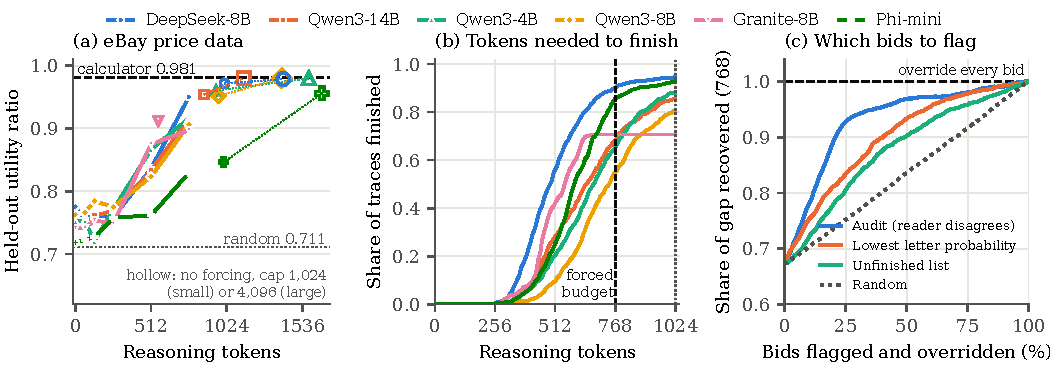
\includegraphics[width=\textwidth]{figures/main_figure_v43.pdf}
\vspace{-3mm}
\caption{(a) Held-out utility ratio by forced budget (filled, 648 decisions per point) and without forcing at mean token use (hollow; small: 1{,}024 cap, large: 4{,}096). (b) Share of all unforced traces that have evaluated every option by token $t$. (c) Share of the 768-token gap recovered when a given share of bids is flagged and overridden with the calculator's bid, by flag, mean over the six models; the audit first flags bids whose answer's written value falls furthest below the largest.}
\label{fig:main}
\Description{Three line plots: utility ratio against reasoning tokens for six models; share of unforced traces that have evaluated every option against tokens; share of the gap recovered against the share of bids flagged for override, for four flagging rules.}
\vspace{-2mm}
\end{figure*}

\begin{table*}[t]
\caption{Gap to the calculator recovered at 768 forced tokens, \% [95\% interval]. $q(0)$, $q(768)$: utility ratio with no reasoning and at 768 tokens. Answer: the model's letter. Closed: the letter read after the reasoning block is closed. Stated: the answer the trace states where it states one, the letter otherwise. 1{,}024 run: the answer without forcing. FP eq.: the answer scored under the first-price equilibrium curve. AuctionNet: the answer at 768 tokens on the second market. Break-even: best expected profit per decision above which 768 tokens pay for themselves. Qwen3-4B and Qwen3-14B match only after rounding and choose different bids in 28\% of decisions.}
\label{tab:main}
\vspace{-2mm}
\small
\setlength{\tabcolsep}{4pt}
\begin{tabular}{lccccccccc}
\toprule
Model & $q(0)$ & $q(768)$ & Answer & Closed & Stated & 1{,}024 run & FP eq. & AuctionNet & Break-even \\
\midrule
DeepSeek-8B & .775 & .950 & 85 [78,92] & 91 [86,95] & 77 [69,85] & 96 [93,98] & 85 [77,92] & 92 [89,95] & 1.78\textcent \\
Phi-mini    & .718 & .829 & 42 [34,50] & 84 [79,88] & 64 [56,71] & 49 [40,57] & 40 [28,49] & 24 [15,32] & 1.71\textcent \\
Qwen3-4B    & .752 & .916 & 72 [66,78] & 72 [63,79] & 73 [66,80] & 91 [87,96] & 74 [69,80] & 80 [75,85] & 1.34\textcent \\
Qwen3-8B    & .763 & .907 & 66 [60,73] & 77 [70,85] & 66 [58,74] & 87 [82,92] & 67 [61,73] & 67 [62,73] & 2.34\textcent \\
Qwen3-14B   & .749 & .916 & 72 [66,78] & 86 [80,92] & 73 [66,80] & 89 [83,94] & 75 [68,81] & 83 [78,87] & 4.49\textcent \\
Granite-8B  & .740 & .897 & 65 [57,73] & 70 [63,76] & 72 [66,77] & 72 [66,77] & 74 [68,80] & 73 [68,78] & 2.19\textcent \\
\bottomrule
\end{tabular}
\vspace{-3mm}
\end{table*}

\begin{table}[t]
\caption{Where the 768-token gap goes, \% of the gap [95\% interval]; rows sum to 100 up to rounding. Letters read with the reasoning block open. Finished: forced traces that evaluate every option. Median: tokens by which half of unforced traces finish, $K=5$/$K=7$. Arithmetic: lower bound (upper bound for Granite-8B: 45, passed over 37). Phi-mini (stated) scores its stated answer. Intervals can dip below zero: a wrong answer can beat the calculator on held-out data.}
\label{tab:traces}
\vspace{-2mm}
\small
\setlength{\tabcolsep}{1.1pt}
\begin{tabular}{lcccccc}
\toprule
Model & Finished & Median & \begin{tabular}[b]{@{}c@{}}Not\\reached\end{tabular} & Arithmetic & Cut off & \begin{tabular}[b]{@{}c@{}}Passed\\over\end{tabular} \\
\midrule
DeepSeek-8B & 90\% & 440/544 & \phantom{0}2 & \phantom{0}5 [0, 17] & 44 [24, 61] & 48 [32, 67] \\
Phi-mini    & 84\% & 544/664 & \phantom{0}5 & \phantom{0}2 [0, 3] & 11 [7, 17] & 82 [74, 89] \\
\ \ (stated) &  &  & \phantom{0}8 & \phantom{0}2 [0, 4] & 18 [11, 26] & 72 [61, 83] \\
Qwen3-4B    & 64\% & 608/776 & 15 & \phantom{0}0 [0, 0] & 63 [51, 73] & 22 [12, 34] \\
Qwen3-8B    & 53\% & 656/840 & 34 & \phantom{0}4 [0, 8] & 39 [29, 50] & 23 [15, 32] \\
Qwen3-14B   & 66\% & 616/704 & 20 & \phantom{0}3 [$-$1, 9] & 59 [49, 70] & 18 [7, 30] \\
Granite-8B  & 71\% & 464/616 & 11 & 22 [13, 32] & \phantom{0}6 [1, 11] & 61 [51, 70] \\
\bottomrule
\end{tabular}
\vspace{-3mm}
\end{table}

\paragraph{Overview}
For every model most of the loss comes after the best option's value is on the page, not from arithmetic. Forcing 768 tokens recovers 42--85\% of the calculator's lead (Table~\ref{tab:main}). In dollars pooled over decisions it recovers 25--75\%. For five models arithmetic is at most 5\% of the gap with the lower bound and 17\% with the upper (Table~\ref{tab:traces}). Shares move by at most 11 points at match tolerances of 1--5\% or under FP eq.

\paragraph{Budget: the Qwen models and DeepSeek-8B}
These models lose mainly to the token cap. Their gap is mostly \emph{not reached} or \emph{cut off} (Table~\ref{tab:traces}), and greedy forced traces at 512 tokens are prefixes of those at 768, so we can watch a list finish: when it does, they answer correctly in 84--89\% of cases. Allowed to stop on their own within 4{,}096 tokens, they rarely hit the cap (at most 1.1\%) and stop after a median of 980--1{,}390 tokens. They then recover 99--100\% of the gap (Figure~\ref{fig:main}a). Those tokens cost 0.45--1.11\textcent{} per decision, while the smallest best expected profit in any scenario (\$1.75) is 39--130 times the break-even at 768 tokens. For these models the fix is not to cap reasoning; asking for every option's profit in the prompt does not help either (Qwen3-8B loses 22 points [14, 31] because its longer lists no longer fit; Phi-mini, Granite-8B and DeepSeek-8B move by at most 5).

\paragraph{Readout: Phi-mini}
Phi-mini's loss is mostly a readout effect: its trace states the right option, but its letter departs from it. A rule-based parser reads the last answer the trace itself states. It agrees with the letter in 96--98\% of Qwen traces but in only 57\% of Phi-mini's. The cause is the readout prompt, which asks for the letter while the reasoning block is still open. When we first close the block with the model's own end-of-thinking marker, Phi-mini's letter agrees with its stated answer in 95\% of decisions and recovers 84\% of the gap (Closed in Table~\ref{tab:main}). Left to close the block itself within 4{,}096 tokens, it recovers 91\% [87, 94] (median 1{,}364 tokens, 6.8\% at the cap). The same change adds 5--14 points for DeepSeek-8B, Granite-8B, Qwen3-8B and Qwen3-14B and nothing for Qwen3-4B.

\paragraph{Decision and arithmetic: Granite-8B}
Granite-8B is the one model whose loss is partly arithmetic; the rest is passing over, and the split depends on the arithmetic bound (Table~\ref{tab:traces}). It is not a readout effect: its stated answer agrees with its letter in 93\% of finished traces, and with the block closed 58\% of its gap is still passed over. Nor is it caused by forcing: on its unforced traces passing over is still 55\% of the gap.

\paragraph{Which wrong bids, and their cost}
Wrong answers lean toward the highest bid on the menu, the one most likely to win. For DeepSeek-8B and the Qwen models it accounts for 40--48\% of wrong answers against about 18\% by chance. The lean is about size, not place in the list: option orders are randomised, and with display position held fixed a wrong answer from these models is far more likely to be the highest bid than any other wrong option (conditional logit, odds ratio 3.9 [2.9, 5.1]; AuctionNet 3.9 [3.2, 4.8]), while being listed first or last makes an option no more likely. The lean survives the closed block (38--45\% of wrong answers) and sampling at temperature 0.6 over five seeds (40--52\%). Nor is it a difficulty effect: in a logistic regression over all models (3{,}519 traces that write the best value and rank it first; errors clustered by scenario), holding the profit gap, position, $K$, value, product and model fixed, passing over is a third as likely when the best option is itself the highest bid (odds ratio 0.36 [0.28, 0.46]). Under pay-your-bid pricing these choices cost bidders 7--17\% of the surplus the calculator's bids earn (\$15k--\$36k per 1{,}000 decisions); for DeepSeek-8B and the Qwen models, 51--78\% of that loss comes from choosing the highest bid. Under eBay's rule, where the winner pays about the closing price, higher bids do not hurt the bidder.

\paragraph{A second market}
The pattern holds on AuctionNet. At 768 tokens the models recover 24--92\% of the gap (Table~\ref{tab:main}), and without forcing DeepSeek-8B and the Qwen models recover 95--98\% within 1{,}024 tokens and 99--100\% within 4{,}096. Closing the reasoning block lifts Phi-mini from 24\% to 81\% [75, 86] and moves the others by 2--15 points. Arithmetic is at most 3\% of the gap for five models and 19\% for Granite-8B; not reached and cut off make up 59--77\% of the Qwen models' gap. Passing over is again much less likely when the best option is the highest bid (odds ratio 0.29 [0.22, 0.38]). The audit, with its reader setting chosen on eBay alone, recovers 86--99\%.

\paragraph{Audit}
Checking the answer against the trace's own numbers catches most errors. The text reader alone does not replace the answer (its gains are in-sample, and it hurts four models on synthetic traces), but as a flag it works: overriding the bids where reader and answer disagree with the calculator's bid recovers 84--100\% of the gap under nested cross-validation, with the reader's settings chosen on the other two products, and also when chosen on synthetic traces only. At every flag rate it beats flags by low letter probability, unfinished lists or chance (Figure~\ref{fig:main}c); flagging 20\% of bids recovers 89\% of the gap against at most 81\%. We do not price the review itself.

\section{Scope and conclusion}
\label{sec:proxy}
Win curves come from eBay prices and one simulated ad market; real ad-exchange logs are untested. Each market has only three products: intervals that also resample products are wider (at 768 tokens, 10--59\% for Phi-mini and 67--99\% for DeepSeek-8B) but stay below the calculator, and arithmetic stays at most 15\% of the gap for five models. The calculator is an oracle; we do not test a model that calls a tool and can fail to. We test open models of up to 14B parameters; whether frontier models also pass over and lean high is untested. For small open reasoning models choosing a bid from a landscape, the loss is mostly not arithmetic but the token cap, the readout prompt (largely fixed by closing the reasoning block) and the final choice. Two findings belong to the models, not our protocol, and survive the closed-block readout: passing over the best option the trace wrote, and the lean toward the highest bid. Flagging answers that disagree with the trace's own numbers recovers most of the loss, and the same check needs no calculator to raise the flag.

\section*{Ethical considerations}
The auction data are a public research dataset of completed eBay listings. Our scenarios use only prices, not the public bidder handles in the source, and we do not redistribute the raw file; AuctionNet is simulated. No human participants were involved.

\bibliographystyle{ACM-Reference-Format}
\bibliography{references}

\end{document}
